%\documentclass[aspectratio=169]{beamer}
\documentclass[aspectratio=169]{beamer} 
% \documentclass{beamer} 
%\documentclass[aspectratio=169,handout]{beamer} 
\setbeameroption{show notes on second screen=bottom}

\usepackage{bigints}

\usepackage{tikz}
\usetikzlibrary{shadows,fadings,calc}

\usepackage{pgfplots}
\pgfplotsset{compat=1.18}
\usepgfplotslibrary{groupplots}

\usepackage{microtype}
\usepackage[style=authoryear-comp,backend=biber]{biblatex}
\addbibresource{biblio.bib}

\usepackage{graphicx}   % graphics
\graphicspath{{./figures/}}

\usepackage{booktabs}

\usepackage{tikz}
\usetikzlibrary{shadows,fadings,calc}

\usepackage{minted}

\tikzfading[name=fade up, bottom color=transparent!0, top color=transparent!100]

\usepackage{appendixnumberbeamer}

\definecolor{wong_blue}{RGB}{0, 114, 178} % #0072B2
\definecolor{wong_orange}{RGB}{230, 159, 0} % #E69F00
\definecolor{wong_green}{RGB}{0, 158, 115} % #009E73
\definecolor{wong_purple}{RGB}{204, 121, 167} % #CC79A7
\definecolor{wong_skyblue}{RGB}{86, 180, 233} % #56B4E9
\definecolor{wong_vermillion}{RGB}{213, 94, 0} % #D55E00
\definecolor{wong_yellow}{RGB}{240, 228, 66} % #F0E442

\hypersetup{colorlinks,linkcolor=,urlcolor=wong_blue,citecolor=wong_purple}

\DeclareMathOperator{\erf}{erf}

\setkeys{Gin}{width=.75\textwidth, height=.75\textheight, keepaspectratio}

\newcommand\blfootnote[1]{%
  \begingroup
  \renewcommand\thefootnote{}\footnote{#1}%
  \addtocounter{footnote}{-1}%
  \endgroup
}

\usepackage{xspace}
\newcommand{\libsvm}{\texttt{libsvm}\xspace}
\newcommand{\x}{{\boldsymbol{x}}}
\newcommand{\y}{{\boldsymbol{y}}}
\newcommand{\z}{{\boldsymbol{z}}}

\usetheme{metropolis}

\pgfplotsset{cycle list={wong_blue,wong_orange,wong_green,wong_purple,wong_skyblue,wong_vermillion,wong_yellow}}

% \setbeamercolor{background canvas}{bg=white}
\setbeamertemplate{caption}[default]

\setbeamercolor{progress bar}{fg=wong_blue,bg=lightgray}

\title{I'll See You In the Limit:}
\subtitle{Understanding the Effects of Infinite Neural Network Kernels}
\date{October 19, 2023}
\author{Aleix Bon\'e}
\institute{
    \textbf{Degree:} Master's Degree in Data Science \\
    \textbf{Thesis supervisor:} Lluís Antonio Belanche-Muñoz (Department of Computer Science)
    \\[2em]
    \textbf{Facultat d’Informàtica de Barcelona (FIB)} \\
    \textbf{Universitat Politècnica de Catalunya (UPC) \textendash{} BarcelonaTech}
}

\titlegraphic{
	\tikz [remember picture,overlay]
	\node at
	([xshift=-3.25cm, yshift=+1.8cm]current page.south east)
	{
\includegraphics[width=0.4\textwidth]{logo-upc}};
}

\begin{document}
\maketitle

\centering

\section{Introduction}

\begin{frame}{Introduction \textendash{} \textcite{frenayParameterinsensitiveKernelExtreme2011}}
	\begin{center}
		\tikz\node [drop shadow]
		{\fcolorbox{black}{white}{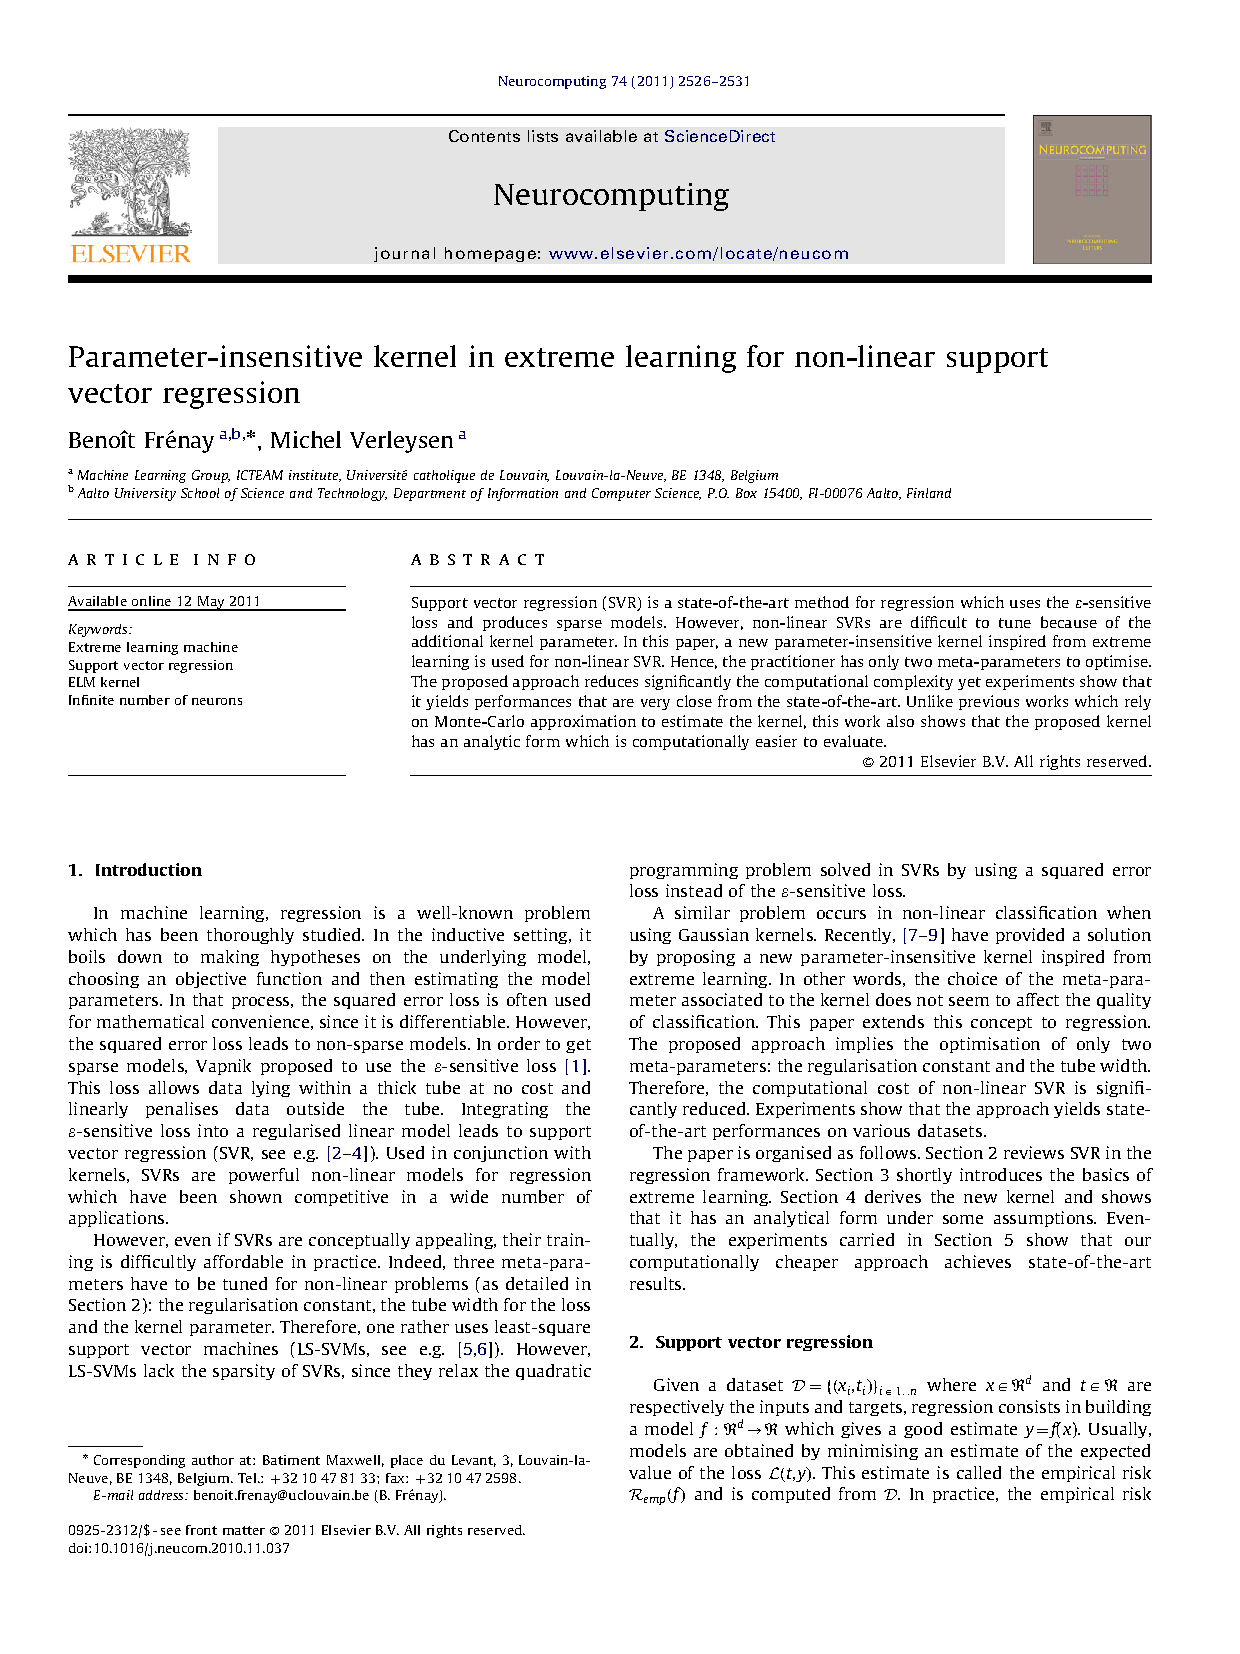
\includegraphics[width=0.8\textwidth,height=!]{frenay_paper}}};
	\end{center}
	\begin{tikzpicture}[overlay,remember picture]
		\coordinate (A) at ($(current page.south east) + (0, 0.5cm)$);
		\fill[color=normal text.bg, path fading=fade up] (current page.west) rectangle ($(A) - (0, 0.01cm)$);
		\fill[color=normal text.bg] (current page.south west) rectangle (A);
	\end{tikzpicture}
	\blfootnote{\fullcite{frenayParameterinsensitiveKernelExtreme2011}}
\end{frame}

\note[itemize]{
	\item \Textcite{frenayParameterinsensitiveKernelExtreme2011} presented a
	``parameter-insensitive'' kernel inspired from extreme learning machines.
	\item The meta-parameter associated with the kernel, once it reaches a certain threshold,
	further increasing its value
	does \emph{not affect} the performance of the results.
	\item They demonstrate effectiveness of the kernel in a Support Vector Regression task.
	\item Not significantly different from \emph{state-of-the-art} using Gaussian kernels.
	\item Seeing these results, we wonder if this property is also present in other
	infinite neural network kernels to some extent.
}

\begin{frame}{Introduction \textendash{} Goals}
	\begin{itemize}
		\item Study the effects of infinite neural network kernels
		\item Focusing on the dependence (or lack of) of performance on the kernel hyperparameters
	\end{itemize}
\end{frame}

\note{
	The aim of this project is to study the effects of these infinite neural network
	kernels in support vector machines; understanding their behaviour in practical
	learning problems, with a special focus on the dependence (or lack of) of
	performance on the kernel
	hyperparameters.

	Having a parameter-insensitive kernel has the potential to cut down on the time
	spent on hyperparameter tuning, which is one of the most time-consuming tasks in
	machine learning.
}

\begin{frame}{Introduction \textendash{} Methodology}
	\begin{enumerate}
		\item Research known infinite neural network kernels in the literature.
		\item Implement the kernels in \libsvm.
		\item Collect suitable datasets.
		\item Design and run experiments.
		\item Analyze the results.
	\end{enumerate}
\end{frame}

\section{Theoretical Background}

\begin{frame}{Theoretical Background \textendash{} Kernel Function}
	A kernel function is a function $k$ that, given two vectors $\boldsymbol x$ and $\boldsymbol y$ in a
	vector space $\mathcal{X}$, returns the inner product of their images in a
	feature space $\mathcal{H}$:
	\begin{equation*}
		k(\boldsymbol x,\, \boldsymbol y) = \left\langle \phi(\boldsymbol x),\, \phi(\boldsymbol y) \right\rangle_{\mathcal{H}}
	\end{equation*}
	where $\phi$ is a mapping from $\mathcal{X}$ to $\mathcal{H}$.
\end{frame}
\note[itemize]{
	\item Such a mapping $\phi$ is called a \emph{feature map}.
	\item $\mathcal{H}$ is an inner product space, and is called the
	\emph{reproducing kernel Hilbert space} (RKHS).
	\item These functions can be used to define a similarity measure.
	\item They can be used in machine learning algorithms such as support vector machines,
	allowing them to operate in a high-dimensional, implicit feature space without
	ever computing the coordinates of the data in that space.
	\item We call learning algorithms that accept kernels \emph{kernel methods}.
}
\begin{frame}{Theoretical Background \textendash{} Single Layer Feed-Forward Neural Network}
	\begin{figure}[htpb]
		% Single layer feedforward network
		\resizebox{.8\textwidth}{!}{
			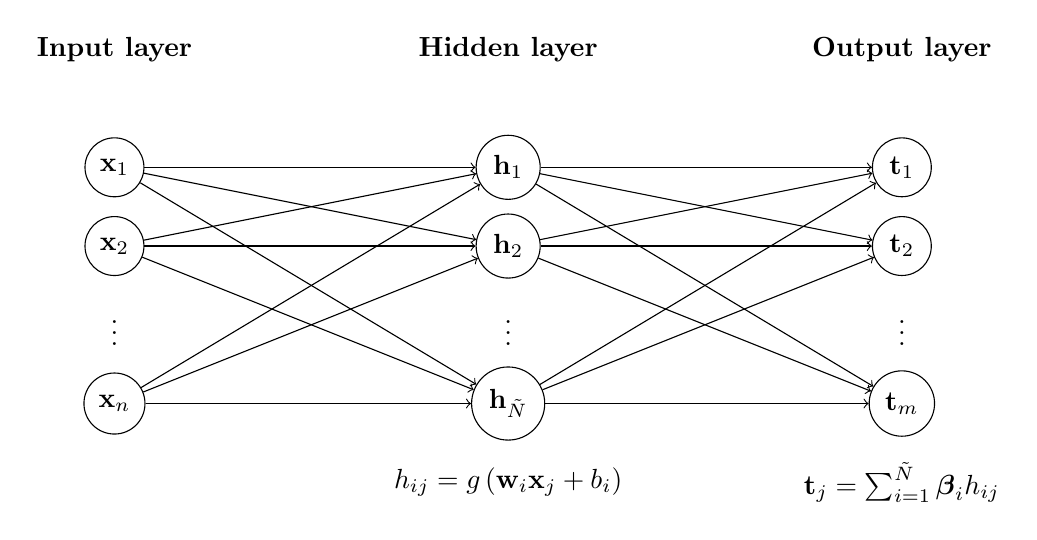
\begin{tikzpicture}
				% input layer
				\node[draw, circle] (x1) at (0, 0) {$\textbf x_1$};
				\node[draw, circle] (x2) at (0, -1) {$\textbf x_2$};
				\node (x3) at (0, -2) {$\vdots$};
				\node[draw, circle] (x4) at (0, -3) {$\textbf x_n$};

				% hidden layer
				\node[draw, circle] (h1) at (5, 0) {$\textbf h_1$};
				\node[draw, circle] (h2) at (5, -1) {$\textbf h_2$};
				\node (h3) at (5, -2) {$\vdots$};
				\node[draw, circle] (h4) at (5, -3) {$\textbf h_{\tilde{N}}$};

				% output layer
				\node[draw, circle] (y1) at (10, 0) {$\textbf t_1$};
				\node[draw, circle] (y2) at (10, -1) {$\textbf t_2$};
				\node (y3) at (10, -2) {$\vdots$};
				\node[draw, circle] (y4) at (10, -3) {$\textbf t_m$};

				\node (xtitle) at (0, 1.5) {\textbf{Input layer}};
				\node (htitle) at (5, 1.5) {\textbf{Hidden layer}};
				\node (ytitle) at (10, 1.5) {\textbf{Output layer}};

				\node (hformula) at (5, -4) {$h_{ij} = g \left( \textbf{w}_i \textbf{x}_j + b_i \right)$};
				\node (yformula) at (10, -4) {$\textbf{t}_{j} = \sum_{i=1}^{\tilde{N}} \boldsymbol\beta_{i} h_{ij}$};

				% connections
				\foreach \i in {1,2,4}
				\foreach \j in {1,2,4} {
						\draw[->] (x\i) -- (h\j);
						\draw[->] (h\i) -- (y\j);
					}
			\end{tikzpicture}
		}
		\caption{Single layer feedforward network}%
	\end{figure}
\end{frame}

\note[itemize]{
	\item $g$ is the activation function, which is applied element-wise to the
	weighted sum of the inputs to the neuron.
	\item $\boldsymbol w_i$ is the weight vector of the $i$-th neuron.
	\item $b_i$ is the bias of the $i$-th neuron.
	\item $\boldsymbol\beta_i$ is the weight vector of the $i$-th output neuron.
}

\begin{frame}{Theoretical Background \textendash{} Activation Function}
	\begin{figure}[H]
		\begin{tikzpicture}
			\begin{groupplot}[group style={
							group size=3 by 1,
							xlabels at=edge bottom,
							ylabels at=edge left,
							vertical sep=4em,
						},
					width = .3\textwidth,
					ymin=-0.1, ymax=1.1,
					every axis plot/.append style={mark=none, line width=2pt},
					enlarge x limits=false,
					samples=25,
					domain=-10:10,
					xmin=-10, xmax=10,
					grid=both,
					grid style={dotted, draw=gray!40, line width=1.0pt}
				]
				\nextgroupplot[title={\bfseries ReLU},xmin=-2,xmax=2]
				\addplot[color=wong_blue] gnuplot[id=relu]{x > 0 ? x : 0};

				\nextgroupplot[title={\bfseries Sigmoid }]
				\addplot[color=wong_orange,smooth] gnuplot[id=sigmoid]{exp(x)/(1 + exp(x))};

				\nextgroupplot[title={\bfseries tanh },ymin=-1,xmin=-5,xmax=5]
				\addplot[color=wong_green,smooth] gnuplot[id=tanh]{tanh(x)};
			\end{groupplot}
		\end{tikzpicture}
		\caption{Activation functions often used in neural networks}
		\label{fig:common_activation_functions}
	\end{figure}
\end{frame}

\begin{frame}{Theoretical Background \textendash{} Extreme Learning Machines (I)}
	Introduced by \textcite{huangExtremeLearningMachine2006}, Extreme Learning
	Machines (ELMs) are an alternative approach to training Single Layer Feed-forward
	Neural Networks (SLFNs):
	\begin{itemize}
		\item Randomly initialize the weights and biases of the hidden layer ($\boldsymbol w_i$ and $b_i$).
		\item Compute the output weights ($\boldsymbol\beta_i$) as: $\boldsymbol\beta = \boldsymbol H^\dagger \boldsymbol T$.
	\end{itemize}
\end{frame}
\note[itemize]{
	\item $\boldsymbol H$ is the hidden layer output matrix, and $\boldsymbol T$ is the target matrix.
	\item $\boldsymbol H^\dagger$ is the Moore-Penrose pseudoinverse of $\boldsymbol H$.
	\item Works with infinitely differentiable activation functions.
}

\begin{frame}{Theoretical Background \textendash{} Extreme Learning Machines (II)}
	\begin{columns}
		\begin{column}{0.4\textwidth}
			\textbf{Pros:}
			\begin{itemize}
				\item Fast training.
				\item Good generalization.
				\item No local minima.
			\end{itemize}
		\end{column}
		\begin{column}{0.4\textwidth}
			\textbf{Cons:}
			\begin{itemize}
				\item No control over the hidden layer.
				\item Underfitting and Overfitting issues.
				\item Dependent on the number of hidden neurons.
			\end{itemize}
		\end{column}
	\end{columns}
\end{frame}
\note{
	Some form of cross-validation is needed to determine the number of hidden neurons.
}


\begin{frame}{Theoretical Background \textendash{} ELM (arcsin) kernel (I)}
	\textcite{frenayParameterinsensitiveKernelExtreme2011} consider a kernel
	in which its feature map $\phi$ is that of an ELM with $p$ hidden nodes and \emph{erf} activation function.
	\begin{columns}
		\begin{column}{0.4\textwidth}
			\begin{align*}
				k(\boldsymbol x,\, \boldsymbol y,\,p) & = \frac{1}{p} \left\langle \phi(\boldsymbol x),\, \phi(\boldsymbol y) \right\rangle_{\mathcal{H}} \\[1em]
				\erf(x)                               & = \frac{2}{\sqrt{\pi}} \int_{0}^{x} e^{-t^2} dt
			\end{align*}
		\end{column}
		\begin{column}{0.6\textwidth}
			\begin{figure}[H]
				\begin{tikzpicture}
					\begin{axis}[
							every axis plot/.append style={smooth, mark=none, line width=1.5pt, domain=-3:3, samples=50, no markers},
							enlarge x limits=false,
							legend pos=north west,
							height=4.5cm,
							width=0.9\textwidth,
							grid=both,
							grid style={dotted, draw=gray!40, line width=1.0pt}
						]
						\addplot+ gnuplot[id=erf]{erf(x)};
						\addlegendentry{$\erf(x)$};
						\addplot+[dashed] gnuplot[id=tanh]{tanh(x)};
						\addlegendentry{$\tanh(x)$};
					\end{axis}
				\end{tikzpicture}
				\caption{\emph{erf} and \emph{tanh} are very similar}
			\end{figure}
		\end{column}
	\end{columns}
\end{frame}

\begin{frame}{Theoretical Background \textendash{} ELM (arcsin) kernel (II)}
	At the limit of $p \to + \infty$, the kernel function is equivalent to the one
	proposed by \textcite{williamsComputingInfiniteNetworks1996} from the context of
	Bayesian Neural Networks (BNNs):
	\begin{equation}
		k(\boldsymbol x,\,\z \mid p \to + \infty)  = \frac{2}{\pi}
		\arcsin \frac{1 + \left\langle \boldsymbol x,\,\z \right\rangle}{\sqrt{
				\left(
				\frac{1}{2\sigma_w^2} + 1 + \left\langle \boldsymbol x,\,\boldsymbol x \right\rangle
				\right)
				\left(
				\frac{1}{2\sigma_w^2} + 1 + \left\langle \z,\,\z \right\rangle
				\right)
			}}
	\end{equation}
	where $\sigma_w^2$ is the variance of the weights \footnote{
		More precisely, $\sigma_w^2$ is the variance of Gaussian distribution with 0 mean from which the weights and biases of the
		hidden layer are drawn.
	}
\end{frame}
\note{
	Where $\sigma_w^2$ is the variance of Gaussian distribution with 0 mean from which the weights and biases of the
	hidden layer are drawn.
}

\begin{frame}{Theoretical Background \textendash{} Arccosine kernel}
	\textcite{choLargemarginClassificationInfinite2010} generalize the work of
	\textcite{williamsComputingInfiniteNetworks1996} by considering alternative activation functions:
	\begin{align*}
		k_n(\boldsymbol x, \y) & = 2 \bigintss \frac{\exp\left(-\frac{\lVert \textbf w \rVert^2}{2}\right)}{(2\pi)^{d/2}}
		\Theta(\textbf w \cdot \boldsymbol x) \Theta(\textbf w \cdot \y) (\textbf w \cdot \boldsymbol x)^n (\textbf w \cdot \y)^n \,d\textbf w \\
		\text{where: }                                                                                                                         \\
		\Theta(z)              & = \frac{1}{2} \bigl(1 + \text{sign}(z)\bigr)
	\end{align*}
\end{frame}

\begin{frame}{Theoretical Background \textendash{} Kernel normalization}
\end{frame}

\section{Conclusions}

\begin{frame}{Conclusions}
	\begin{itemize}%[<+->]
		\item TODO
	\end{itemize}
\end{frame}

\begin{frame}[standout]
	Thank you!
\end{frame}

\begin{frame}{Outline}
	\vspace{1em}
	\tableofcontents
\end{frame}
% Add extra slides for presentation
\appendix

%bibilio
\begin{frame}[allowframebreaks]{References}
	\printbibliography[heading=none]
\end{frame}

\begin{frame}[standout]
	Extra slides
\end{frame}

\end{document}
